%===============================================================================
% LaTeX sjabloon voor de bachelorproef toegepaste informatica aan HOGENT
% Meer info op https://github.com/HoGentTIN/bachproef-latex-sjabloon
%===============================================================================

\documentclass{bachproef-tin}

\usepackage{hogent-thesis-titlepage} % Titelpagina conform aan HOGENT huisstijl

%%---------- Documenteigenschappen ---------------------------------------------
% TODO: Vul dit aan met je eigen info:

% De titel van het rapport/bachelorproef
\title{Titel}

% Je eigen naam
\author{Steven Stevens}

% De naam van je promotor (lector van de opleiding)
\promotor{Jan Janssens}

% De naam van je co-promotor. Als je promotor ook je opdrachtgever is en je
% dus ook inhoudelijk begeleidt (en enkel dan!), mag je dit leeg laten.
\copromotor{Piet Pieters}

% Indien je bachelorproef in opdracht van/in samenwerking met een bedrijf of
% externe organisatie geschreven is, geef je hier de naam. Zoniet laat je dit
% zoals het is.
\instelling{---}

% Academiejaar
\academiejaar{2018-2019}

% Examenperiode
%  - 1e semester = 1e examenperiode => 1
%  - 2e semester = 2e examenperiode => 2
%  - tweede zit  = 3e examenperiode => 3
\examenperiode{2}

%===============================================================================
% Inhoud document
%===============================================================================

\begin{document}

%---------- Taalselectie -------------------------------------------------------
% Als je je bachelorproef in het Engels schrijft, haal dan onderstaande regel
% uit commentaar. Let op: de tekst op de voorkaft blijft in het Nederlands, en
% dat is ook de bedoeling!

%\selectlanguage{english}

%---------- Titelblad ----------------------------------------------------------
\inserttitlepage

%---------- Samenvatting, voorwoord --------------------------------------------
\usechapterimagefalse
%%=============================================================================
%% Voorwoord
%%=============================================================================

\chapter*{\IfLanguageName{dutch}{Woord vooraf}{Preface}}
\label{ch:voorwoord}

%% TODO:
%% Het voorwoord is het enige deel van de bachelorproef waar je vanuit je
%% eigen standpunt (``ik-vorm'') mag schrijven. Je kan hier bv. motiveren
%% waarom jij het onderwerp wil bespreken.
%% Vergeet ook niet te bedanken wie je geholpen/gesteund/... heeft




%%=============================================================================
%% Samenvatting
%%=============================================================================

% TODO: De "abstract" of samenvatting is een kernachtige (~ 1 blz. voor een
% thesis) synthese van het document.
%
% Deze aspecten moeten zeker aan bod komen:
% - Context: waarom is dit werk belangrijk?
% - Nood: waarom moest dit onderzocht worden?
% - Taak: wat heb je precies gedaan?
% - Object: wat staat in dit document geschreven?
% - Resultaat: wat was het resultaat?
% - Conclusie: wat is/zijn de belangrijkste conclusie(s)?
% - Perspectief: blijven er nog vragen open die in de toekomst nog kunnen
%    onderzocht worden? Wat is een mogelijk vervolg voor jouw onderzoek?
%
% LET OP! Een samenvatting is GEEN voorwoord!

%%---------- Nederlandse samenvatting -----------------------------------------
%
% TODO: Als je je bachelorproef in het Engels schrijft, moet je eerst een
% Nederlandse samenvatting invoegen. Haal daarvoor onderstaande code uit
% commentaar.
% Wie zijn bachelorproef in het Nederlands schrijft, kan dit negeren, de inhoud
% wordt niet in het document ingevoegd.

\IfLanguageName{english}{%
\selectlanguage{dutch}
\chapter*{Samenvatting}
\iffalse \lipsum[1-4] \fi
\selectlanguage{english}
}{}

%%---------- Samenvatting -----------------------------------------------------
% De samenvatting in de hoofdtaal van het document

\chapter*{\IfLanguageName{dutch}{Samenvatting}{Abstract}}

\iffalse \lipsum[1-4] \fi

Voor dit onderzoek 


%---------- Inhoudstafel -------------------------------------------------------
\pagestyle{empty} % Geen hoofding
\tableofcontents  % Voeg de inhoudstafel toe
\cleardoublepage  % Zorg dat volgende hoofstuk op een oneven pagina begint
\pagestyle{fancy} % Zet hoofding opnieuw aan

%---------- Lijst figuren, afkortingen, ... ------------------------------------

% Indien gewenst kan je hier een lijst van figuren/tabellen opgeven. Geef in
% dat geval je figuren/tabellen altijd een korte beschrijving:
%
%  \caption[korte beschrijving]{uitgebreide beschrijving}
%
% De korte beschrijving wordt gebruikt voor deze lijst, de uitgebreide staat bij
% de figuur of tabel zelf.

\listoffigures
\listoftables

% Als je een lijst van afkortingen of termen wil toevoegen, dan hoort die
% hier thuis. Gebruik bijvoorbeeld de ``glossaries'' package.
% https://www.overleaf.com/learn/latex/Glossaries

%---------- Kern ---------------------------------------------------------------

% De eerste hoofdstukken van een bachelorproef zijn meestal een inleiding op
% het onderwerp, literatuurstudie en verantwoording methodologie.
% Aarzel niet om een meer beschrijvende titel aan deze hoofstukken te geven of
% om bijvoorbeeld de inleiding en/of stand van zaken over meerdere hoofdstukken
% te verspreiden!

%%=============================================================================
%% Inleiding
%%=============================================================================

\chapter{\IfLanguageName{dutch}{Inleiding}{Introduction}}
\label{ch:inleiding}

\section{\IfLanguageName{dutch}{Probleemstelling}{Problem Statement}}
\label{sec:probleemstelling}

Dit onderzoek vindt zijn oorsprong in de aloude concurrentie tussen analoge en digitale geluidsverwerking. Meer bepaald bij muzikanten, muzikaal artiesten en producenten die hun \textbf{live} opstelling uitrusten met allerlei analoge componenten. Denk hier aan effectpedalen, voorversterkers, equalizers, compressors, mengpanelen, \textit{Direct Injection} boxen (DI-box) etc. Een productontwerper of IT-bedrijf zou al snel denken om hier digitale varianten van op de markt te brengen. Dat was inderdaad het geval voor veel mengtafelproducenten. Bekende merken zoals AKAI, Roland en Behringer zijn er al in geslaagd om volledig digitale mengtafels te produceren. Veel andere, ook kleinere bedrijven volgen hen. De digitale concurrenten hebben tal van voordelen op hun analoge voorgangers en wekken dus een grote vraag op in bij de consumenten.

Wat onveranderd gebleven is, is de aankoopprijs. Evenals hun analoge voorgangers kosten de digitale mengtafels al makkelijk \EUR{20.000}. Dit onderzoek wilt nog een stap verder gaan met de digitalisering. Deze paper probeert te achterhalen of zulke producten onder te brengen zijn in de vorm van puur software zonder bijkomende hardware. De aankoopprijs kan zo significant dalen en consumenten voeren alle operaties uit met enkel een standaard laptop.

\iffalse
De inleiding moet de lezer net genoeg informatie verschaffen om het onderwerp te begrijpen en in te zien waarom de onderzoeksvraag de moeite waard is om te onderzoeken. In de inleiding ga je literatuurverwijzingen beperken, zodat de tekst vlot leesbaar blijft. Je kan de inleiding verder onderverdelen in secties als dit de tekst verduidelijkt. Zaken die aan bod kunnen komen in de inleiding~\autocite{Pollefliet2011}:

\begin{itemize}
  \item context, achtergrond
  \item afbakenen van het onderwerp
  \item verantwoording van het onderwerp, methodologie
  \item probleemstelling
  \item onderzoeksdoelstelling
  \item onderzoeksvraag
  \item \ldots
\end{itemize}


\section{\IfLanguageName{dutch}{Probleemstelling}{Problem Statement}}
\label{sec:probleemstelling}

Uit je probleemstelling moet duidelijk zijn dat je onderzoek een meerwaarde heeft voor een concrete doelgroep. De doelgroep moet goed gedefinieerd en afgelijnd zijn. Doelgroepen als ``bedrijven,'' ``KMO's,'' systeembeheerders, enz.~zijn nog te vaag. Als je een lijstje kan maken van de personen/organisaties die een meerwaarde zullen vinden in deze bachelorproef (dit is eigenlijk je steekproefkader), dan is dat een indicatie dat de doelgroep goed gedefinieerd is. Dit kan een enkel bedrijf zijn of zelfs één persoon (je co-promotor/opdrachtgever).

\fi

\section{\IfLanguageName{dutch}{Afbakening}{Demarcation}}
\label{sec:afbakening}

De focus ligt puur op de vraag van de consument, de mogelijkheid tot intrede in de markt en de technische realiseerbaarheid.

\subsection{In-scope}

Het onderzoek beperkt zich tot een marktonderzoek en een technische test.

Om te zien of de overstap van analoog naar deze digitale omgeving realistisch is, wordt de technische test uitgevoerd. Daarin worden \textbf{real-life cases} uit de wereld van muziekproductie omgezet naar een \textbf{virtuele omgeving}.

De virtuele omgeving bestaat uit drie libraries voor geluidsverwerking. De libraries worden getest op performantie. Goede resultaten geven aan dat het technisch gezien realistisch is om de overstap naar digitaal te maken.

De real-life cases worden verkregen door middel van interviews in het marktonderzoek. Hier werden bands en producers gevraagd om de opstelling van hun live installaties uit te leggen. Deze installaties worden omgezet naar parameters voor de virtuele test cases. De parameters van de test cases zijn dus een discrete dataset en geen alomvertegenwoordigend spectrum van alle mogelijke installatiescenario's. Dit omdat het testen van een continue dataset teveel tijd in beslag zou nemen (na berekening blijkt 1275 dagen) en omdat meer dan de helft van de test cases redundant zouden zijn.

\subsection{Out-of-scope}

Het is duidelijk dat bij het onderbrengen van analoge producten in een software-pakket, de fysieke user-interface volledig wegvalt. Een fysieke interface is een groot argument pro analoog maar geen geldig argument tegen de potentie van digitalisatie. Daarom valt ergonomie buiten de scope van dit onderzoek.

\iffalse

\section{\IfLanguageName{dutch}{Methodologie}{Methodology}}
\label{sec:methodologie}

Zoals eerder vermeld wordt er een marktonderzoek en technische test uitgevoerd. Deze worden verder in het artikel respectievelijk vernoemd als de emotionele en empirische test.

De emotionele test gaat aan de hand van interviews de maat nagaan waarin of de muzieksector de digitalisatie verwelkomt. Voor de interviews werd gezocht naar muzikanten, bands, muzikaal artiesten, producers en opnamestudio's. De test beantwoordt of er vraag is naar digitalisatie en wie er baat bij zou hebben. Dit onderzoek beschouwt ook de live muziekinstallatie van de artiesten en een paar real-life usecases die ze daarvoor konden geven.

De emotionele test heeft twee uitkomsten: ...

\fi

\section{\IfLanguageName{dutch}{Onderzoeksvragen}{Research questions}}
\label{sec:onderzoeksvragen}

De hoofdvraag luidt als volgt:

\subsubsection{Waarom blijft de muziekindustrie analoog werken in een digitale wereld?}

Secundaire bronnen geven al snel een antwoord op deze vraag. Het antwoord is hetzelfde voor veel vakken die hun overstap van analoog op digitaal maken. Dat blijkt uit de artikels \textit{Analog vs. Digital Synthesizers – My Take on the Old Debate} \autocite{juliusdobos} en \textit{Analogue artists defying the digital age} \autocite{GuardianOpinion} alsook uit de interviews die voor dit onderzoek gevoerd werden. Daarin vonden we terug dat het grootste argument pro analoog de authentieke look-and-feel van de hardware is. Desondanks is dit geen tegenargument voor digitalisatie. Om hier dieper op in te gaan hebben we volgende deelvragen gesteld.

\subsubsection{Is het mogelijk om digitaal te gaan?}

Er zijn al tal van programma's waarmee men live aan geluidsverwerking kan doen. Deze programma's worden vaak gebruikt door DJ's en berusten altijd op externe harware. Deze deelvraag toont aan of de usecase van de DJ gegeneraliseerd kan worden naar andere actoren e.g. bands, producers, opname-artiesten etc.

Er wordt door middel van een literatuurstudie gezocht naar methodes voor digitale geluidsgeneratie en -verwerking. Van hoog belang is dat de methodes real-time toegepast kunnen worden door het doelpubliek; artiesten en producers.

\subsubsection{Is het nuttig om digitaal te gaan?}

Van alle mogelijke methodes voor digitale geluidsverwerking zal de scope vernauwd worden op slechts één methode. Deze methode wordt gekozen op basis van de mate waarin het intuïtief bruikbaar is voor en door het doelpubliek, de real-time capaciteit en de design capaciteit voor het modelleren van geluid.
Zo beantwoordt deze vraag hoe de emotionele en empirische tests opgesteld zullen worden.

\subsubsection{Is het realistisch om digitaal te gaan?}

Op basis van de gekozen methode en hiervoor omschreven requirements worden drie libraries gezocht. Vervolgens worden er door middel van interviews naar real-life usecases gevraagd uit de muzieksector. En als laatste worden de specificaties van het teststation omschreven.

De real-life cases worden generiek omschreven in de libraries. De libraries zullen de cases uitvoeren en worden hierbij getest op performantie. Als er significant goede resultaten zijn, zelfs bij slechts één van de libraries, toont dat aan dat het technisch mogelijk is om digitaal te gaan. De empirische tests worden per usecase uitgevoerd. De resultaten van een test tonen enkel aan dat het realistisch is om digitaal te gaan voor die specifieke usecase.

Dit is de empirische test.

\subsubsection{Is de overstap van analoog naar digitaal mogelijk?}

Naast real-life usecases worden de geïnterviewden ook gevraagd in welke mate ze de digitalisatie verwelkomen en of ze geïnteresseerd zouden zijn in zulke innovaties.

Dit is de emotionele test.

Op basis van de resultaten van zowel de emotionele als empirische tests wordt per usecase bepaald of het mogelijk is om de overstap naar digitaal te maken.

\iffalse

Wees zo concreet mogelijk bij het formuleren van je onderzoeksvraag. Een onderzoeksvraag is trouwens iets waar nog niemand op dit moment een antwoord heeft (voor zover je kan nagaan). Het opzoeken van bestaande informatie (bv. ``welke tools bestaan er voor deze toepassing?'') is dus geen onderzoeksvraag. Je kan de onderzoeksvraag verder specifiëren in deelvragen. Bv.~als je onderzoek gaat over performantiemetingen, dan 

\fi

\section{\IfLanguageName{dutch}{Onderzoeksdoelstelling}{Research objective}}
\label{sec:onderzoeksdoelstelling}

De emotionele en empirische tests hebben elk twee uitkomsten: positief en negatief. Afhankelijk van de resultaten van de tests kunnen ondernemingen beslissen of het slim is om de markt te betreden met deze innovatie.

\subsection*{Emotionele test}

\begin{itemize}
    \item \textbf{Positief}: Uit de interviews blijkt dat de muzieksector geïnteresseerd is in digitalisering. Een onderneming kan succesvol deze markt betreden.
    \item \textbf{Negatief}: Deze innovatie wordt niet verwelkomd door de muzieksector. Wanneer een onderneming deze markt betreedt zal het geen vruchten afwerpen.
\end{itemize}

\subsection*{Empirische test}

\begin{itemize}
    \item \textbf{Positief}: Deze usecase is uitvoerbaar op het teststation. Het is technisch gezien mogelijk voor de actor om de overstap naar digitaal te maken.
    \item \textbf{Negatief}: Deze usecase is niet uitvoerbaar op het teststation. De actor van de usecase moet een sterkere machine hebben of blijft beter analoog te werk gaan.
\end{itemize}

\iffalse

Wat is het beoogde resultaat van je bachelorproef? Wat zijn de criteria voor succes? Beschrijf die zo concreet mogelijk. Gaat het bv. om een proof-of-concept, een prototype, een verslag met aanbevelingen, een vergelijkende studie, enz.

\fi

\section{\IfLanguageName{dutch}{Opzet van deze bachelorproef}{Structure of this bachelor thesis}}
\label{sec:opzet-bachelorproef}

% Het is gebruikelijk aan het einde van de inleiding een overzicht te
% geven van de opbouw van de rest van de tekst. Deze sectie bevat al een aanzet
% die je kan aanvullen/aanpassen in functie van je eigen tekst.

De rest van deze bachelorproef is als volgt opgebouwd:

Hoofdstuk \ref{ch:stand-van-zaken} geeft de setting van dit onderzoek weer. De manieren om dit onderzoek te benaderen en de reeds gevoerde onderzoeken in datzelfde domein

In Hoofdstuk~\ref{ch:methodologie} wordt de methodologie toegelicht en worden de gebruikte onderzoekstechnieken besproken om een antwoord te kunnen formuleren op de onderzoeksvragen.

% TODO: Vul hier aan voor je eigen hoofstukken, één of twee zinnen per hoofdstuk

In Hoofdstuk~\ref{ch:conclusie}, tenslotte, wordt de conclusie gegeven en een antwoord geformuleerd op de onderzoeksvragen. Daarbij wordt ook een aanzet gegeven voor toekomstig onderzoek binnen dit domein.
\chapter{\IfLanguageName{dutch}{Stand van zaken}{State of the art}}
\label{ch:stand-van-zaken}

% Tip: Begin elk hoofdstuk met een paragraaf inleiding die beschrijft hoe
% dit hoofdstuk past binnen het geheel van de bachelorproef. Geef in het
% bijzonder aan wat de link is met het vorige en volgende hoofdstuk.

% Pas na deze inleidende paragraaf komt de eerste sectiehoofding.

\section{Inhoud}

In het hoofdstuk \ref{ch:inleiding}: \nameref{ch:inleiding} werd al gesproken over interviews, methodes voor geluidsgeneratie en libraries voor geluidsverwerking. In dit hoofdstuk zullen alledrie die onderwerpen verder uiteengezet worden. Deze onderwerpen vormen de primaire en een deel van de secundaire bronnen van dit onderzoek.

\section{Interviews}

TO DO:
\begin{itemize}
    \item Push interviews naar git.
    \item Transcribe.
    \item hoofdpunten noteren per interview.
\end{itemize}{}

\subsection{Correspondentie}

\subsection{Bart Vincent}

\subsection{Peter Boone}

\subsection{Thomas Houthave}

\subsection{Vagabundos}

\section{Methodes voor Geluidsgeneratie en -verwerking}

%\textcite{methodes} beschrijft in zijn boek vijf methodes digitale geluidsgeneratie en toepassingen ervan.

\begin{itemize}
    \item Subtractive Synthesis
    \item Additive Synthesis
    \item Granular Synthesis
    \item Wavelet en Corpus-based Synthesis
\end{itemize}{}

De werking van deze methodes wordt hieronder verder toegelicht.

\subsection{Subtractive Synthesis}

Bij subtractive synthesis start de gebruiker met een harmonisch rijke geluidsgolf. Een golf is harmonisch rijk wanneer het veel subfrequenties bevat. Voorbeelden hiervan zijn zaagtand-, blok- en driehoeksgolven Wanneer de golf puur gehoord wordt zal de fundamentele frequentie het dominantst klinken \autocite{harmonics}. Het is de taak van de gebruiker om door middel van frequentiefilters de ongewenste delen van het frequentiespectrum weg te halen en zo het geluid te modelleren \autocite{subtractive}

\textcite{subtractive} bespreken in hun artikel methodes voor digitale geluidsgeneratie en -verwerking. Deze methodes zijn slechts een benadering van wat analoge synthesizers doen. Maar in tegenstelling tot andere pogingen om analoge geluidsgeneratie te digitaliseren zijn de resultaten van deze methodes niet te onderscheiden van het analoge geluid \autocite{subtractive}.

Subtractive synthesis is tot vandaag nog steeds de standaard voor geluidsdesign sinds Robert A. Moog de eerste subtractive synthesizer modules uitbracht in de jaren '60 \autocite{subtractive}. \textcite{guitarpedals} beschrijft in zijn artikel hoe sommige effecten, die vandaag terug te vinden zijn in de effectpedalen voor gitaristen, digitaal verwerkt kunnen worden; allemaal door middel van subtractive synthesis.

\subsection{Additive Synthesis}

Additive synthesis is de tegenhanger van subtractive synthesis. Sinusgolven staan er gekend om maar één frequentie te hebben; hun fundamentele frequentie. Bij additive synthesis gaat de gebruiker tal van sinusgolven bij elkaar optellen om complexere geluiden te bekomen \autocite{additive}.

Voor kleine toepassingen is deze berekening nog haalbaar voor een digitale workstation. Maar van het moment dat de geluiden complexer en harmonisch rijker moeten zijn, loopt de doorlooptijd van de generatie linear op met het aantal sommen van de additieve golf \autocite{additive}.

Wanneer men harmonisch rijke golven wilt genereren zoals de zaagtandgolf, is dit onmogelijk te volbrengen op additieve wijze door het oneindig aantal sommaties dat berekend moet worden \autocite{harmonics}.

\subsection{Granular Synthesis}

Bij granular synthesis start de gebruiker met een of meerdere zeer korte geluidsfragmenten - grains - die aanzien worden als een periode van een geluidsgolf. De gebruiker zal die periode verschillende keren kopiëren en verschalen. De periode krijgt vervolgens ook een aanvangsttijd toegewezen. Door verschillende grains op die manier met elkaar te vermengen, kan de gebruiker het gewenste geluid modelleren \autocite{granular}.

Granular synthesis is van eigen al een techniek die enkel digitaal toegepast kan worden. Met de IT-sector als doelpubliek is het een zeer aantrekkelijke methode voor sound synthesis. De techniek is zeer bruikbaar voor geluidssimulaties en -imitaties, vooral door middel van een AI \autocite{granular}.

\textcite{granular} legt in zijn paper zelfs een manier uit om in real-time (live) aan granulair geluid te genereren. Zelf geeft hij aan het einde van zijn artikel wel toe dat hij geen toekomst ziet voor granular synthesis in de muziekproductie. Dit omdat er teveel parameters zijn die de gebruiker moet beïnvloeden.

\subsection{Wavelet en Corpus-based Synthesis}

Deze twee generatie methodes zijn soorten van granular synthesis. Door hun verschil in implementatie zijn ze elk toepasbaar op andere vlakken.

\subsubsection{Wavelet Synthesis}

Wavelet synthesis biedt de gebruiker niet meerdere maar slechts één periode om het modelleerproces mee te starten. De periode, hier wavelet genoemd, is op voorhand specifiek gekozen door de gebruiker om het gewenste geluid te kunnen bekomen. Verder verloopt het modelleerproces volledig zoals granular synthesis \autocite{wavelet}.

Deze methode wordt meer gebruikt wanneer men zeer gedetailleerd geluid wilt nabootsen. Het modeleerproces vereist dat de gebruiker een goed inzicht heeft in muziektheorie en vergt ook dat het geluid iteratief gemodeleerd wordt 
\autocite{wavelet}. Real-time is het dus slecht toepasbaar.

\subsubsection{Corpus-based Granular Synthesis}

Deze granulaire generatiemethode haalt de grains op uit een databank - de corpus - van vooraf opgenomen geluiden. Deze methode wordt vooral gebruikt wanneer men een specifiek geluid wilt imiteren. Een zoekalgoritme of AI weet dan exact waar hij gelijkaardige grains terug kan vinden en probeert dan het originele geluid na te bootsen aan de hand van die grains 
\autocite{methodes}.

Corpus-based is niet toepasbaar wanneer de gebruiker nieuwe geluiden wilt maken. Niet alleen heeft het dezelfde tekortkomingen als gewone granulaire geluidsgeneratie, het heeft ook nog extra vrijheidsgraden van welke grains te kiezen uit de hele corpus.

\section{Libraries}

\subsection{JASS}

\textcite{jass} ontwikkelden JASS (Java Audio Synthesis System) voor hun onderzoek naar efficiente geluidsgeneratie. Deze library synthetiseert zeven voorafgaande onderzoeken naar modellen voor geluidsgeneratie die bedoeld zijn voor geluidseffecten in video games en simulaties. 

\textcite{jass} leggen uit hoe verschillende libraries verschillende doeleinden, implementaties en kosten hebben. Hun doel met JASS is om een library te schrijven die, naast alle requirements die opgelijst staan in hun paper, ook een breed scala van mogelijke toepassingen heeft. JASS is dus bedoeld als all-round library voor om het even welke sector \autocite{jass}.

\subsubsection*{De Code}
\label{sec:jass_code}

JASS kan teruggevonden worden op de website van van den Doel \autocite{jasscode}.

In hun paper leggen \textcite{jass} de innerlijke werking van JASS uit. Hier valt op dat het een modulaire\footnote{Iedere module heeft zijn eigen atomaire rol (oscillator, filter, compressor, versterker etc.). Door ze met elkaar te verbinden - of patchen - krijgt de gebruiker een zelf ontworpen stramien van parameters waarmee hij zijn geluid kan boetseren.} library is. De ontwikkelaar kan zijn eigen modules ontwikkelen door over te erven van gegeven abstracte klassen en interfaces  \autocite{jass}. 

Dit is ook hoe programma's voor geluidsbewerking en (modulaire) synthesizers opgebouwd zijn. Modulaire programma's zijn intuïtief voor gebruikers uit de muzieksector \autocite{bartvincent}.

Een ontwikkelaar instantieert een geluidsgenererende subklasse. Deze klasse erft dus van de \verb+Out+ klasse. Bijgevolg moet deze klasse de \verb+computeBuffer+ methode implementeren. Deze methode kan twee dingen doen. Ofwel genereert het een buffer. Ofwel verwerkt het een buffer die de klasse verkrijgt via een \verb+Source+ attribuut. Alle klassen die erven van \verb+In+ en \verb+InOut+ hebben een \verb+addSource+ methode waarmee een \verb+Source+ toegevoegd kan worden \autocite{jass}.

Wanneer een stramien van verwerkte buffers uiteindelijk via een \verb+SourcePlayer+ aangesloten wordt op de audio output van de machine, kan de buffer gehoord worden. Evenals subklassen van \verb+In+ en \verb+InOut+ kan een \verb+SourcePlayer+ meerdere \verb+Source+'s hebben \autocite{jass}.

\subsection{Beads}

Beads is een open-source Java library gemaakt door Oliver Bown. Het project is in 2008 tot stand gekomen met behulp van Monash University in Melbourne en heeft in 2014 zijn laatste update gekregen \autocite{beads}.

De library is bedoeld voor het schrijven van real-time\footnote{Wanneer een library of programma multi-threaded werkt zodat de gebruiker met het geluid kan interageren terwijl het gegenereerd of bewerkt wordt.} programma's voor geluidsverwerking. Java was hier onmiddellijk de taal van voorkeur omdat het open-source is. De ontwikkelaars melden op hun site dat ze een zeer flexibele IO-laag geïmplementeerd hebben. De library functioneert zo in verschillende contexten \autocite{beads}. 

Het doel van Beads is het vergemakkelijken audio-implementatie. Bown en zijn team hopen om de ontwikkeling van audio applicaties toegankelijker te maken voor de standaard programmeur \autocite{beads2}.

\subsubsection*{De Code}

Programmeren in Beads start met het instantiëren van een \verb+AudioContext+. Deze klasse vraagt in zijn constructor naar een audio output device. Het selecteren van een audio output device is mogelijk in native Java \autocite{beadsdocs}.

Beads biedt een paar reeds voorgeprogrammeerde oscillatoren aan. Deze zijn ondergebracht in de \verb+Buffer+ klasse. De golven kunnen afgespeeld worden met de \verb+WavePlayer+ klasse \autocite{beadsdocs}.

Beads werkt, net zoals JASS, ook modulair. Klassen die erven van \verb+UGen+ implementeren de \verb+addInput+ methode. De methode vraagt een andere \verb+UGen+ als parameter wiens output de input wordt van de betreffende \verb+UGen+ \autocite{beadsdocs}.

Om \verb+UGen+'s te horen, moeten ze aangesloten worden op de \verb+AudioContext+. De \verb+AudioContext+ kan meerdere \verb+UGen+'s als input aanvaarden. Vervolgens moet de ontwikkelaar de \verb+start+ methode oproepen in \verb+AudioContext+ om het geluid af te laten spelen \autocite{beadsdocs}.

\subsection{JSyn}

JSyn is - de naam verraadt het - een Java library die traditionele modellen van modulaire synthesizers imiteert \autocite{jsyn}. Net zoals Beads is het real-time en open-source verkrijgbaar op GitHub \autocite{jsyngit}.

Mobileer Inc. hebben naast JSyn ook twee andere software audio projecten gereleased: JMSL (Java Music Specification Language) en PortAudio. JMSL is een Java-based specificatie taal waarin gebruikers instrumenten en composities kunnen definiëren. PortAudio is een cross-platform audio IO-library voor C \autocite{jsyn}.

\subsubsection*{De Code}

Beschouw de documentatie van JSyn \autocite{jsyndocs}. Daar vinden we een aantal herkenbare klassen terug zoals basis oscillatoren (sinus-, zaagtand-, driehoeks- en blokgolf), verschillende soorten filters (low-pass, high-pass, band-pass, multi-pole etc.) en zelfs effecten (delay, envelope etc.).

JSyn baseert zich op één moederklasse: \verb+Synthesizer+. Wanneer een ontwikkelaar modules instantieert, moeten die via de \verb+add+ methode toegevoegd worden aan de \verb+Synthesizer+ vooraleer ze gehoord kunnen worden. De \verb+Synthesizer+ klasse staat in voor het starten van alle toegevoegde modules en beslist ook de geluidskwaliteit van de output \autocite{jsyndocs}.

De genererende en verwerkende klassen hebben - net zoals in JASS - een methode die een buffer genereert of verwerkt. Kijk hiervoor terug naar \ref{sec:jass_code}. De methode heet \verb+pullData+ en verkrijgt de te verwerken buffers via de \verb+UnitInputPort+-attributen van de klassen \autocite{jsyndocs}.

JSyn is, evenals Beads en JASS ook modulair. Het verbinden van klassen is mogelijk door de \verb+UnitInputPort+- en \verb+UnitOutputPort+-attributen van genererende en verwerkende klassen. Via de \verb+connect+ methode kan een ontwikkelaar een \verb+UnitOutputPort+ connecteren aan een \verb+UnitInputPort+ \autocite{jsyndocs}.

Een stramien van verwerkte buffers, wordt via de \verb+LineOut+ klasse op de audio output van de machine aangesloten. Wanneer de ontwikkelaar de \verb+start+ methode oproept op zowel de \verb+LineOut+ als de \verb+Synthesizer+, weerklinkt het geluid. Het \verb+UnitInputPort+-attribuut van \verb+LineOut+ kan meerdere inputs ontvangen \autocite{jsyndocs}.

\subsection*{Vergelijking van de Libraries}

\begin{longtable}[c]{l|lll}
         & \textbf{Beads} & \textbf{JASS} & \textbf{JSyn} \\ \hline
        \textbf{Real-time} & Ja & Ja & Ja \\
        \textbf{Modulair} & Ja & Ja & Ja \\
        \textbf{Buffer methode} & calculateBuffer & computeBuffer & pullData \\
        \textbf{Synthesis methode} & Subtractive & Subtractive & Subtractive \\
    \caption{Vergelijking van de drie testlibraries.}
    \label{tab:vergelijking}
\end{longtable}

Wanneer we de documentatie van de drie libraries beter bekijken, valt op dat hun code in essentie hetzelfde doet. Niet alleen hebben ze alle gelijkenissen uit tabel \ref{tab:vergelijking}, de architectuur van het verbinden van genererende en verwerkende buffers is duidelijk ook typerend aan sound libraries.

Uitzonderlijk bij JSyn is wel dat alle parameters een \verb+UnitInputPort+ zijn. Neem een low-pass filter (LPF) als voorbeeld. Gegeven een harmonisch rijke geluidsgolf gaat een LPF alle aanwezige frequenties hoger dan een gegeven cut-off frequentie weg filteren. Het te filteren geluid is hier de input - bij zowel JSyn als andere libraries is dit het geval. De cut-off frequentie is hier een parameter voor de module.\newline
Bij de meeste libraries zijn zulke parameters statische getallen. JSyn behandelt zulke parameters als \verb+UnitInputPort+'s \autocite{jsyndocs}.

De filosofie van object-oriented programming is het modelleren van de echte wereld. In dit voorval is JSyn de beste representatie van echte modulaire synthesizers. Parameters van modules zijn maar zelden statische waarden. Artiesten willen een interactieve band hebben met hun geluid. Daarvoor moeten zulke parameters dynamisch aangepasbaar zijn \autocite{vagabundos}. In het geval van modulaire synthesizers \textit{"moduleert"} men parameters door middel van \textit{"control voltage"} \autocite{modular}.

\iffalse

Dit hoofdstuk bevat je literatuurstudie. De inhoud gaat verder op de inleiding, maar zal het onderwerp van de bachelorproef *diepgaand* uitspitten. De bedoeling is dat de lezer na lezing van dit hoofdstuk helemaal op de hoogte is van de huidige stand van zaken (state-of-the-art) in het onderzoeksdomein. Iemand die niet vertrouwd is met het onderwerp, weet nu voldoende om de rest van het verhaal te kunnen volgen, zonder dat die er nog andere informatie moet over opzoeken \autocite{Pollefliet2011}.

Je verwijst bij elke bewering die je doet, vakterm die je introduceert, enz. naar je bronnen. In \LaTeX{} kan dat met het commando \texttt{$\backslash${textcite\{\}}} of \texttt{$\backslash${autocite\{\}}}. Als argument van het commando geef je de ``sleutel'' van een ``record'' in een bibliografische databank in het Bib\LaTeX{}-formaat (een tekstbestand). Als je expliciet naar de auteur verwijst in de zin, gebruik je \texttt{$\backslash${}textcite\{\}}.
Soms wil je de auteur niet expliciet vernoemen, dan gebruik je \texttt{$\backslash${}autocite\{\}}. In de volgende paragraaf een voorbeeld van elk.

\textcite{Knuth1998} schreef een van de standaardwerken over sorteer- en zoekalgoritmen. Experten zijn het erover eens dat cloud computing een interessante opportuniteit vormen, zowel voor gebruikers als voor dienstverleners op vlak van informatietechnologie~\autocite{Creeger2009}.

\lipsum[7-20]

\fi

%%=============================================================================
%% Methodologie
%%=============================================================================

\chapter{\IfLanguageName{dutch}{Methodologie}{Methodology}}
\label{ch:methodologie}

%% TODO: Hoe ben je te werk gegaan? Verdeel je onderzoek in grote fasen, en
%% licht in elke fase toe welke stappen je gevolgd hebt. Verantwoord waarom je
%% op deze manier te werk gegaan bent. Je moet kunnen aantonen dat je de best
%% mogelijke manier toegepast hebt om een antwoord te vinden op de
%% onderzoeksvraag.

\section{Inhoud}

Allereerst worden de \textbf{empirische tests} uitgevoerd. Deze tests gaan na of de digitalisatie mogelijk is op technisch vlak. Het doel van dit onderzoek is analoge apparatuur om te vormen in pure software zodat het toegankelijker is voor consumenten met een lager budget. Daarom werd voor de technische tests gebruik gemaakt van een standaard particulieren laptop. De code geschreven voor de uitvoering van de tests wordt samen met de specificaties van het testsysteem respectievelijk besproken in secties \ref{subsec:methodologie:code} en \ref{subsec:methodologie:testmachine}.

Zodat de testcases van de empirische tests representatief zouden zijn, werd er gezocht naar real-life usecases uit de muzieksector. Hiervoor zijn interviews afgenomen. De interviews zelf zijn besproken in sectie \ref{sec:interviews}. In de interviews werden artiesten, producers etc. gevraagd naar hun opstellingen voor zowel in opname als voor live muziek. Aan hand van die informatie werden representatieve testcases opgesteld. De opstelling van de testcases staan uitgelegd in sectie \ref{subsec:methodologie:code}. 

In de interviews werd ook gevraagd of digitale varianten verwelkomd zouden worden op de markt. Dit is interessant voor software bedrijven die de muzieksector willen betreden. Als er wel degelijk vraag is naar zulke innovaties, weten zij dat het voordelig is om in die niche te gaan werken. Hoe de antwoorden van de interviewees verwerkt werden staat beschreven in sectie \ref{sec:methodologie:emotioneletests}. Dit zijn de \textbf{emotionele tests}.

\section{Empirische tests}
\label{sec:methodologie:empirischetests}

\subsection{De Testmachine}
\label{subsec:methodologie:testmachine}

Er werd gezocht naar een laptop met gemiddelde specificaties voor de hedendaagse markt. Als deze laptop de testcases al aankan dan geldt hetzelfde voor andere gemiddelde particuliere laptops en zeker voor workstations van opnamestudio's en backstage geluidstechnici.

De gekozen machine is een Lenovo Ideapad Flex-14. Het modelnummer is 20308. De specificaties van de machine staan in tabel \ref{tab:specmachine}. Op de machine draaide een verse installatie van Linux Mint Sylvia.

\begin{table}[]
\centering
\begin{tabular}{lll}
\hline
\multicolumn{3}{c}{\textbf{Component}}                \\ \hline
\textbf{Type} & \textbf{Naam}       & \textbf{Kracht} \\ \hline
Processor     & Intel Core i3-4010U & 1.70GHz         \\ \hline
RAM           & DDR3L SDRAM         & 8,00 GB         \\ \hline
Opslag        & Hybride Drive       & 500 GB
\end{tabular}
\caption{Specificaties van de Testmachine}
\label{tab:specmachine}
\end{table}

\subsection{De Code}
\label{subsec:methodologie:code}

\subsubsection{Keuze en Werking van de Libraries}

Uit de interviews, besproken in sectie \ref{sec:interviews}, bleek dat de muzieksector altijd met subtractive synthesis werkt bij hun geluidsgeneratie en -verwerking. Voor de empirische tests zijn dus drie subtractive sound synthesis libraries gekozen. Zoals vermeld in sectie \ref{sec:libraries} zijn dit Beads, JASS en JSyn.

Sectie \ref{subsec:vergelijkinglibraries} toont aan dat de drie libraries in essentie een gelijkaardige werking hebben. Iedere oscillator en geluidsverwerkende klasse voert een specifieke bewerking uit op een buffer. De buffers kunnen ook aan elkaar geconnecteerd worden; de output van de buffer wordt de input van een andere. Zo maakt de gebruiker een stramien van parameters die hij kan gebruiken om het geluid te modeleren.

\subsubsection{Opstelling van de Testcases}

De testcases zijn opgesteld aan de hand van de interviews. De interviewees werden gevraagd naar volgende specificaties van hun opstelling. 

\begin{itemize}
	\item Hoeveel audiosporen er gebruikt worden.
	\item Op hoeveel van die sporen equalization en compressie van toepassing is.
	\item Het aantal effecten dat op eenzelfde moment actief is op een spoor.
	\item Op hoeveel van die sporen het stramien van effecten actief staat.
	\item Hoeveel parameters ze op één moment moeten bedienen.
\end{itemize}

Het aantal sporen werd in code vertaald naar oscillatoren. Die oscillatoren werden geconnecteerd aan equalizers en compressors. Die output werd - indien van toepassing - ook geconnecteerd aan een stramien van effecten. Alle losse outputs van oscillatoren, compressors en effecten werden aangesloten op de audio output lijn van het programma. Op die manier konden de antwoorden weergegeven worden als volgende vier integere parameters.

\begin{itemize}
	\item Het aantal oscillatoren.
	\item Het aantal oscillatoren dat geconnecteerd wordt aan een equalizer en compressor.
	\item Het aantal effecten.
	\item Het aantal oscillatoren dat - eventueel na hun connectie aan een compressor - aan een stramien van effecten geconnecteerd wordt.
\end{itemize}

Voor het opstellen van de testcases is rekening gehouden met hoeveel buffers berekend worden in het programma. De testcases worden per library uitgevoerd in stijgende volgorde van het aantal gebruikte buffers. De paramerters staan per profiel weergegeven in tabellen \ref{tab:profielen} en \ref{tab:parameters}.

\begin{table}[]
\begin{tabular}{ll|c}
\textbf{Interviewee} & \textbf{Profiel} & \textbf{Testcase index} \\ \hline
- & Hobbyist & 1 \\
Vagabundos \& Peter Boone & Live band & 2 \\
Vagabundos \& Peter Boone & Band in opname & 3 \\
Saulo Soneghet & Metal band in opname & 4 \\
Bart Vincent & Jazz band in concert & 5 \\
Thomas Houthave & Sound designer & 6 \\ \hline
\end{tabular}
\caption{Testcase index per profiel}
\label{tab:profielen}
\end{table}

\begin{table}[]
\begin{tabular}{c|cccc|c}
\textbf{Index} & \textbf{\#Tracks} & \textbf{\#EQ en compressie} & \textbf{\#Effecten} & \textbf{\#Tracks met effecten} & \textbf{\#Buffers} \\ \hline
1 & 4 & 4 & 0 & 0 & 4 \\
2 & 10 & 10 & 2 & 5 & 40 \\
3 & 25 & 25 & 2 & 10 & 95 \\
4 & 40 & 40 & 3 & 15 & 165 \\
5 & 50 & 50 & 5 & 20 & 250 \\
6 & 150 & 150 & 0 & 0 & 450 
\end{tabular}
\caption{Testcase parameters per index}
\label{tab:parameters}
\end{table}

\subsubsection{Architectuur en Werking van de Test Framework}

De code voor het uitvoeren van de testcases is terug te vinden in appendix \ref{ch:code}.

De volgende taak was om een test framework te maken. Met de parameters geformuleerd in tabel \ref{tab:parameters}, moet het framework library-specifieke testcases uitvoeren en de performantie meten van het proces. Er werd rekening gehouden met uitbreidbaarheid zodat andere libraries makkelijk toegevoegd kunnen worden. Daarvoor werd de template pattern toegepast.

\begin{figure}
  \centering
    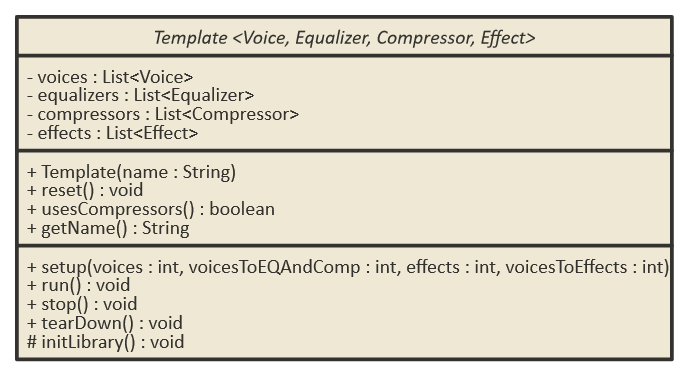
\includegraphics[width=0.5\textwidth]{imgs/nomnoml.png}
  \caption{Klasse diagram van de Template klasse}
  \label{fig:template}
\end{figure}

Figuur \ref{fig:template} toont het klasse diagram van de abstracte en generieke \verb+Template+ klasse van het framework. Dit is de moederklasse van de library specifieke testklasses. Wanneer een klasse zich uitbreid op \verb+Template+, representeert de subklasse een sound synthesis library. De subklasse moet eerst de generieke types \verb+Voice+, \verb+Equalizer+, \verb+Compressor+ en \verb+Effect+ definiëren.

\begin{itemize}
	\item \textbf{Voice} is een oscillatorklasse uit de library.
	\item \textbf{Equalizer} is een klasse uit de library die een inkomende buffer verwerkt. Om trouw te blijven aan de real-life testcases gebruikt men hier best een geluidsfilter. Geluidsfilters hebben karakteristieken van equalizers.
	\item \textbf{Compressor}: idem aan \textbf{Equalizer}.
	\item \textbf{Effect} is nog een verwerkende klasse. Deze klasse representeert een geluidseffect. Bart Vincent en Vagabundos gebruikten vaak een delay effect. \autocite{bartvincent} \autocite{vagabundos} Het wordt aangeraden om een gelijkaardig effect uit de library te kiezen.
\end{itemize}

 In de subklasse worden vervolgens de \verb+setup+-, \verb+run+-, \verb+stop+- en \verb+tearDown+-methode overgeërft. Deze worden als volgt ingevuld.

\begin{itemize}
	\item \textbf{Setup} vraagt de vier parameters uit tabel \ref{tab:parameters}. Aan de hand van deze parameters worden de \verb+Voice+-, \verb+Equalizer+-, \verb+Compressor+-, \verb+Effect+-modules correct geïnstantieerd, geconnecteerd en opgeslagen in de desbetreffende attributen uit de \verb+Template+-klasse.
	\item De \textbf{run}-methode start alle oscillatoren en verwerkende modules die in de \verb+setup+-methode opgesteld zijn. Sound synthesis libraries starten in de meeste gevallen automatisch een nieuwe thread wanneer dit gebeurt. Als dit niet het geval is, moet de ontwikkelaar het zelf in een thread laten uitvoeren\footnote{JASS start bijvoorbeeld geen nieuwe thread wanneer SourcePlayer.start() opgeroepen wordt. Om dit op te lossen werd de PlayThread-klasse ontworpen die de SourcePlayer eenmalig start tot de halt methode opgeroepen wordt.}. Dit is belangerijk voor de performantiemeting. 
	\item De \textbf{stop}-methode stopt de thread - en bijgevolg ook het geluid - die in de \verb+run+-methode opgeroepen is.
	\item \textbf{TearDown} haalt de opstelling van de testcase terug uit elkaar. Voor de modules verwijderd kunnen worden uit het geheugen, moeten ze eerst veilig gedeconnecteerd worden van zowel de library als van de andere componenten. Zo kan de library terug volledig geïnitialiseerd worden voor de volgende testcase.
\end{itemize}

De uit te voeren testklassen en de parameters van de testcases worden statisch bijgehouden in de \verb+StartUp+-klasse. In de \verb+main+-methode wordt per testklasse iedere testcase uitgevoerd. Tijdens het runnen van de audio thread, wordt de performantie van het proces gemeten.

\subsubsection{Performantiemeting van het Proces}

Het voordeel van in een Linux-omgeving te werken is dat er geen externe library nodig is voor de performantiemeting. Alle nodige informatie kan al verkregen worden via het \verb+top+-commando. De taak voor het afnemen van de metingen werd in het framework aan de \verb+Measurer+-klasse gegeven. In die klasse kan commando \ref{command} teruggevonden worden.

\begin{figure}
\centering
\begin{verbatim}
	top -b -n1 -d,01 | \\
	grep %d | \\
	awk '{ if (\$9 != \"0,0\") print \$9 \" \" \$10 }'
\end{verbatim}
\caption{Linux commando om performantie van een proces te meten.}
\label{command}
\end{figure}

\verb+Top+ is een real-time commando. Wanneer het opgeroepen wordt in de terminal, worden alle processen en hun verbruik van CPU en geheugen dynamisch weergegeven. \autocite{topcommand} De volgende vlaggen worden toegepast.

\begin{itemize}
	\item \textbf{-b} start het proces in \textit{Batch mode}. Dit zorgt dat de header met algemene infromatie niet afgebeeld wordt zodat de output beter verwerkt kan worden door andere programma's of commando's.
	\item \textbf{-n1} maakt maar één meting in plaats van een continue dynamische output te geven.
	\item \textbf{-d,01} voert de meting op 0,01 seconden uit.
\end{itemize}

De \verb+-n+-vlag wordt gebruikt omdat Java geen output van dynamische commando's kan lezen. De \verb+-d+-vlag wordt gebruikt zodat de enkele meting zo snel mogelijk gemaakt wordt. Zo doende dook er een probleem op. Wanneer \verb+top+ standaard uitgevoerd wordt, update het proces ongeveer iedere de seconde. Wanneer men de metingen frequenter uit voert, wordt vastgesteld dat de meting voor \verb+%CPU+ onleesbaar is. Ongeveer iedere seconde wordt er een geldige meting afgebeeld. Daartussen vertoont de meting een \verb+0+ als resultaat.

Het interval van de seconde is niet betrouwbaar; soms was het meer, soms was het minder. Daarom wordt iedere 0,01 seconden een meting genomen. Ongeldige metingen worden genegeerd door het programma. Andere metingen worden opgeslaan tot er een totaal van 50 metingen per testcase is. Iedere meting duurt nog steeds ongeveer een seconde, maar van het moment dat een geldige meting verkrijgbaar is, wordt die ook opgenomen. 

De output van het \verb+top+-commando wordt doorgegeven aan het \verb+grep+-commando. Java String formatting maakt gebruik van de \verb|"%d"| om de \textit{process ID} van het framework in te voeren in het commando. Zo verkrijgt men een enkele meting van het gezochte proces. \verb+StartUp+ heeft een statische methode \verb+getPID()+ die de \textit{process ID} van het framework teruggeeft. De output van \verb+grep+ wordt doorgegeven aan het \verb+awk+-commando.

Het \verb+awk+-commando filtert de \verb+%CPU+ en \verb+%Mem+ meting uit de output van \verb+grep+ op voorwaarde dat de \verb+%CPU+-meting geldig is. De output van dit commando wordt ingelezen door Java. De twee metingen worden nog gescheiden door een spatie zodat het makkelijk te verwerken is.

\subsection{Verwerking van de Testresultaten}
\label{sec:methodologie:verwerking}

Per library is er een dataset van 6 testcases. Iedere testcase heeft een subset van 50 metingen. Op zo'n subset wordt eerst een dubbele \textit{moving median} uitgevoerd. \autocite{mediansmoothing} Dit is een smoothing methode waarbij twee keer een nieuwe dataset gemaakt wordt. De nieuwe dataset wordt bekomen door een item te vervangen door de mediaan van zichzelf, zijn voorganger en zijn nakomer; zoals getoond in berekening \ref{math:mediansmooth}. $y_{i}$ is het item van de nieuwe dataset en $x$ representeert de oude dataset. De eerste en laatste waarden worden overgenomen uit de oude dataset omdat berekening \ref{math:mediansmooth} niet mogelijk is op die indexen. Deze dubbele smoothing verwijdert korte periodes van extrema.

\begin{figure}
\centering
$y_{i} = med(x_{i-1}, x_{i}, x_{i+1})$
\caption{\textit{Moving median} formule}
\label{math:mediansmooth}
\end{figure}

De resulterende dataset wordt vervolgens gladgestreken door middel van de Hanning vensterfunctie. Deze functie maakt dat plotse variaties in het frequentiedomein geëgaliseerd worden. Op die manier komen waarden die frequenter voorkomen in de dataset dominanter naar voor. Dit door het lopend gewogen gemiddelde van de waarden in de dataset te berekenen. De Hanning van een waarde in een dataset wordt berekend als de helft van die waarde opgeteld met een kwart van de voorgaande en nakomende meting. Dit staat afgebeeld in berekening \ref{math:hanningformule}. De eerste en laatste waarden van de nieuwe dataset worden overgenomen uit de oude dataset. \autocite{hanning}

\begin{figure}
\centering
$h_{i} = (y_{i-1} + 2 \ast y_{i} + y_{i+1}) \div 4$
\caption{Hanning formule}
\label{math:hanningformule}
\end{figure}

Van de resulterende dataset wordt de mediaan genomen als resultaat voor de testcase. De mediaan is niet gevoelig aan extrema en geeft een betere representatie van de meer frequente metingen in een dataset. \autocite{median} Van de medianen wordt een trendlijn berekend. Zolang de richtingscoëfficient van de trendlijn van de testresultaten niet hoger ligt dan die van het aantal buffers in de input parameters uit tabel \ref{tab:parameters}, kunnen we zeggen dat het technisch aanvaardbaar is om een overstap naar digitaal te maken. 

\section{Emotionele tests}
\label{sec:methodologie:emotioneletests}

Na de technische bespreking van de muzikale opstellingen van de interviewees, werden volgende vragen gesteld:

\begin{itemize}
	\item Is er potentie voor digitalisering in de muziekindustrie?
	\item Wie zou hier het meeste baat bij hebben?
	\item Wie zou hier het meeste interesse in hebben?
	\item Zou een digitalisering verwelkomd worden in de sector?
\end{itemize}

Op basis van deze vragen, weten we of de branche van dat profiel in de muzieksector open staat voor een digitalisatie.

Er zijn door tijdsgebrek en de kleine respons (zie tabel \ref{table:correspondentie}) slechts vier interviews afgenomen. Dit is duidelijk te weinig data om een populatie te representeren.

Iedere interviewee beeld een profiel uit zoals in tabel \ref{tab:profielen} staat. Als resultaat op de emotionele test van een profiel wordt uit belang van dit onderzoek het resultaat van de interviewee zelf genomen.

\iffalse \lipsum[21-25] \fi



% Voeg hier je eigen hoofdstukken toe die de ``corpus'' van je bachelorproef
% vormen. De structuur en titels hangen af van je eigen onderzoek. Je kan bv.
% elke fase in je onderzoek in een apart hoofdstuk bespreken.

%\input{...}
%\input{...}
%...

%%=============================================================================
%% Conclusie
%%=============================================================================

\chapter{Conclusie}
\label{ch:conclusie}

% TODO: Trek een duidelijke conclusie, in de vorm van een antwoord op de
% onderzoeksvra(a)g(en). Wat was jouw bijdrage aan het onderzoeksdomein en
% hoe biedt dit meerwaarde aan het vakgebied/doelgroep? 
% Reflecteer kritisch over het resultaat. In Engelse teksten wordt deze sectie
% ``Discussion'' genoemd. Had je deze uitkomst verwacht? Zijn er zaken die nog
% niet duidelijk zijn?
% Heeft het onderzoek geleid tot nieuwe vragen die uitnodigen tot verder 
%onderzoek?

\section{Is het mogelijk om digitaal te gaan?}

Uit sectie \ref{onderzoeksvraag1} bleek dat het wel degelijk mogelijk zou zijn om digitaal te gaan. Er bestaat al technologie voor, het moet enkel nog correct geïmplementeerd worden. De correcte implementatie is hier van essentie, zoals bij de testresultaten van JASS te zien was.

Dat niet alleen. Op dit moment wordt er meer onderzoek gevoerd naar toepassingen van andere methodes van digitale geluidsgeneratie zoals granular en wavelet synthesis. Houthave zei in zijn interview: \textit{``granulaire synthesis is dan weer muzikaler van aard. Daar definieer je instrumenten.''} \autocite{thomashouthave} Dit onderzoek heeft zich beperkt tot subtractive synthesis omdat het de meest intuïtieve generatie- en verwerkingsmethode is voor het doelpubliek. \textcite{granular} legt in zijn paper een methode voor real-time granular synthesis uit. Zoals in sectie \ref{methode:granular} staat moet hier een groot aantal parameters bediend worden dat toeneemt naargelang de complexiteit van het geluid. Daarbij is \textit{simplicity key} voor een product dat aan de consument verkocht wordt. Hier kan zeker verder onderzoek gevoerd worden.

User interfaces vallen buiten de scope van dit onderzoek. Voor verdere ontwikkeling is belangerijk dat de profielen live slechts één parameter op eenzelfde moment bedienen. Met toetsenbord en muis is het zeker haalbaar om de bediening van één parameter uit te voeren.

\section{Is het nuttig om digitaal te gaan?}

Sectie \ref{onderzoeksvraag2} toonde aan dat alle profielen een digitale transitie zouden verwelkomen. Wat opvalt is dat sommige profielen bepaalde eisen stellen voor het eindproduct. Zo eisen muzikanten om het taktiele in hun instrument te behouden en hebben producers nood aan een hogere geluidsresolutie dan standaard CD-kwaliteit. Zolang aan die wensen voldaan kan worden, is er interesse naar digitalisatie op de markt.

Of de consumenten er direct positief op gaan reageren is een ander verhaal. Vincent en Boone zien veel potentieel in digitale verwerking voor live muziek. Voornamelijk omdat digitaal het werkproces versnelt en vergemakkelijkt. Toch blijft Boone sceptisch over de digitale transitie. Ten eerste omdat de genres van zijn klanten niet thuis horen in een digitaal milieu en ten tweede omdat de digitale tafels van vandaag geen deftige geluidsresolutie kunnen verwerken. Er is dus zeker vraag naar digitale mengtafels die hogere geluidsresoluties dan \textit{standaard CD-kwaliteit} \autocite{peterboone} aankunnen.

Uit andere interviews en uit \ref{onderzoeksvraag1} bleek echter dat er geen hoorbaar verschil is tussen digitaal en analoog. Natuurlijk zal analoge verwerking altijd wat ruis en vuil hebben. Sommige artiesten en producers zijn hier net naar opzoek. \textit{``Iemand kan vinden dat digitaal veel cleaner is. Anderen vinden dat ze karakter missen. Maar veel van dat "vuil" kan ook gegenereerd worden door een plugin,''} vertelt Vincent over digitale of analoge voorkeuren. \autocite{bartvincent} 

Boone vertelt na zijn interview over een fout die hij in een track van de Beatles gehoord heeft. Het is algemeen geweten dat er zich veel foutjes in de albums van de Beatles verschuilen. Dat zijn dingen die niet meer kunnen in de muzieksector van vandaag. Een song moet een afgewerkt product zijn, zonder vuil of fouten. Daar kan digitaal zeker bij helpen, zegt Boone. \textit{``Dat is wel een voordeel van digitaal ten opzichte van analoog. Als je bij analoog een te laag opnameniveau hebt en je trekt het op, dan trek je ook de ruis op. En digitaal heeft geen ruis.''} \autocite{peterboone}

Een andere manier om deze vraag te beantwoorden is door te kijken naar de voordelen die digitaal ten opzichte van analoog heeft.

\begin{itemize}
	\item Het opslaan van instellingen en die met een druk op de knop terug kunnen inladen.
	\item Het standaardiseren van die digitale instellingen zodat ze tussen opstellingen en artiesten gedeeld kunnen worden.
	\item De prijs die significant lager ligt in vergelijking met de analoge varianten.
	\item De compactheid van het product.
	\item Digitaal is \textit{cleaner} en bevat geen ruis.
\end{itemize}

Hieruit wordt geconcludeerd dat het algemeen zeker nuttig is om digitaal te gaan. Maar daarmee is niet aan de wensen van ieder profiel voldaan. In sectie \ref{endeontwikkelaars} wordt hier dieper op ingegaan.

\section{Is het realistisch om digitaal te gaan?}
\label{conclusie3}

Om deze vraag te beantwoorden moest slechts één van de libraries een goede performantie vertonen. Pas dan mocht gezegd worden dat het realistisch is om digitaal te gaan. In sectie \ref{onderzoeksvraag3} werd aangetoond dat JSyn alle testcases aankon. Dus wordt geconcludeerd dat het realistisch is om digitaal te gaan.

Voor een open-source Java library heeft JSyn goed gescoord op de empirische test. Maar wanneer puntje bij paaltje komt, zal het eindproduct niet met JSyn geschreven worden. Bedenk dat de empirische tests afgenomen zijn op een particuliere laptop. De laptops verkrijgbaar op de hedendaagse markt zijn veel sterker dan onze testmachine. Bedenk hoe een C++-library zou presteren. Zulke low-level programmeertalen presteren zeker beter dan Java.  

\section{Wat wilt dit zeggen voor ontwikkelaars?}
\label{endeontwikkelaars}

\begin{table}[]
\begin{tabular}{l|l|l|l|}
\cline{3-4}
\multicolumn{2}{l}{\multirow{2}{*}{}}  & \multicolumn{2}{c|}{\textbf{Empirische tests}}                                                                                                                  \\ \cline{3-4} 
\multicolumn{2}{l}{}   & \textbf{Positief} & \textbf{Negatief} \\ \hline
\multicolumn{1}{|l|}{\multirow{2}{*}{\textbf{Emotionele tests}}} & \textbf{Positief} & Betreed de markt.                                                                           & \begin{tabular}[c]{@{}l@{}}Er is interesse maar\\ het is technisch niet mogelijk.\end{tabular} \\ \cline{2-4} 
\multicolumn{1}{|l|}{}                                           & \textbf{Negatief} & \begin{tabular}[c]{@{}l@{}}Het is technisch mogelijk\\ maar weinig vraag naar.\end{tabular} & \begin{tabular}[c]{@{}l@{}}Slecht idee om de markt\\ te betreden.\end{tabular}                 \\ \hline
\end{tabular}
\caption{Uitkomsten van de Emotionele-Empirische test.}
\label{EEtest}
\end{table}

Tabel \ref{EEtest} geeft beter inzicht in de situatie. JSyn scoorde positief op onze empirische tests. In sectie \ref{conclusie3} wordt besproken dat alternatieve manieren van geluidsgeneratie en -verwerking betere prestaties opleveren. Het is technisch zeker mogelijk om de overstap naar digitaal te maken. De emotionele tests, daarentegen, zijn afhankelijk van profiel tot profiel. Waar de digitalisatie gegeerd is voor sound designers, geluidstechnici en sommige muzikanten, is dat niet altijd het geval bij producers en opname artiesten.

Het is technisch zeker mogelijk om de digitale transitie te maken. Uit de interviews bleek bovendien dat daar ook interesse voor is. Dus als hier verdere ontwikkelingen gebeuren - rekening houdend met profielspecifieke requirements - maakt de ontwikkelaar kans in de markt.

\section{Toekomstig Onderzoek}

\subsection{Grotere Bevraging}

Dit onderzoek geeft een duidelijke indicatie dat er ruimte is voor ontwikkelaars in de markt. Een bredere bevraging van de muzieksector is wenselijk om de requirements van de profielen te verfijnen.

\subsection{Proof-of-concept}

Toekomstig onderzoek kan proberen om digitale versies te maken van analoge apparatuur. Denk hierbij aan mengpanelen, voorversterkers, effectpedalen, synthesizers, direct input boxes etc. Bij voorkeur worden deze in een low-level programmeertaal geschreven, onafhankelijk van een library en met een minimalistische user interface.

\subsection{Alternatieve Methodes voor Geluidsgeneratie en -verwerking}

In sectie \ref{sec:methodesgeneratie} werden verschillende methodes voor geluidsgeneratie en -verwerking besproken. Met name granular, wavelet en corpus-based granular synthesis. Toekomstig onderzoek kan op zoek gaan naar efficiente manieren om deze methodes toe te passen in verwerking en generatie van muziek. Dat niet alleen. Thomas Houthave sprak in zijn interview over toepassingen van AI in het simuleren en immiteren van geluid. Hier ziet hij tepassingen voor in sound design voor game engines. \autocite{thomas houthave} Hij sprak ook over \textit{bionische muzikanten} die jammen met een artiest. Het programma speelt in op noten of akkoorden die de muzikant speelt. Zo kan de muzikant begeleid worden in het creëren van zijn muziek.

\iffalse \lipsum[76-80] \fi



%%=============================================================================
%% Bijlagen
%%=============================================================================

\appendix
\renewcommand{\chaptername}{Appendix}

%%---------- Onderzoeksvoorstel -----------------------------------------------

\chapter{Onderzoeksvoorstel}

Het onderwerp van deze bachelorproef is gebaseerd op een onderzoeksvoorstel dat vooraf werd beoordeeld door de promotor. Dat voorstel is opgenomen in deze bijlage.

% Verwijzing naar het bestand met de inhoud van het onderzoeksvoorstel
\input{../voorstel/voorstel-inhoud}

%%---------- Andere bijlagen --------------------------------------------------
% TODO: Voeg hier eventuele andere bijlagen toe
%\input{...}

%%---------- Referentielijst --------------------------------------------------

\printbibliography[heading=bibintoc]

\end{document}
